\section{Experimentos realizados y resultados obtenidos}
\subsection{Experimento con el Perceptrón}
\label{subsec:perceptronexperiment}

El experimento que hemos realizado con el perceptrón ha sido sencillo, con el objetivo de comprobar que el funcionamiento era el esperado y, sobre todo, ver gráficamente como el PLA iba evolucionando los pesos y cual iba siendo la evolución. La función que hemos intentado aproximar con el perceptrón ha sido la función AND, la cual se describe en el algoritmo \ref{alg:andfunction}.

\begin{algorithm}[H]
    
    \eIf{$a * b == 1$}
    {
        $return$ 1$;$
    }
    {
        $return$ 0$;$
    }

	\caption{Función AND}
	\label{alg:andfunction}
\end{algorithm}

La función AND es linealmente separable, por lo que el perceptrón debería de poder separar los puntos eventualmente. En la figura \ref{fig:andFunctionTargets} se muestran los puntos que queremos separar (como subindice tienen el valor que se espera por el perceptrón).

\begin{figure}[h]
	\centering
	\includegraphics[width=1\textwidth]{{"Figures/Perceptrón. Targets"}.png}
	\caption{Puntos de la función AND}
	\label{fig:andFunctionTargets}
\end{figure}

En la figura \ref{fig:andFunctionPLAIterations} podemos ver como el PLA ha ido ajustando los pesos para buscar el plano que separa correctamente estos puntos.

\begin{figure}
\begin{tabular}{cc}
  \includegraphics[width=65mm\textwidth]{{"Figures/Perceptrón. PLA - 1st iteration"}.png} &  \includegraphics[width=65mm\textwidth]{{"Figures/Perceptrón. PLA - 2nd iteration"}.png} \\
1a iteración PLA (25\% acierto) & 2a iteración PLA (75\% acierto) \\[6pt]
 \includegraphics[width=65mm\textwidth]{{"Figures/Perceptrón. PLA - 3rd iteration"}.png} &   \includegraphics[width=65mm\textwidth]{{"Figures/Perceptrón. PLA - 4th iteration"}.png} \\
3a iteración PLA (75\% acierto) & 4a iteración PLA (50\% acierto) \\[6pt]
\includegraphics[width=65mm\textwidth]{{"Figures/Perceptrón. PLA - 5th iteration"}.png} &   \includegraphics[width=65mm\textwidth]{{"Figures/Perceptrón. PLA - 6th iteration"}.png} \\
5a iteración PLA (75\% acierto) & 6a iteración PLA (50\% acierto) \\[6pt]
\multicolumn{2}{c}{\includegraphics[width=65mm\textwidth]{{"Figures/Perceptrón. PLA - 7th iteration"}.png} }\\
\multicolumn{2}{c}{7a iteración PLA (100\% acierto)}
\end{tabular}
\caption{Iteraciones del PLA para la función AND}
\label{fig:andFunctionPLAIterations}
\end{figure}

\newpage

Algo interesante que podemos observar con este experimento es que el porcentaje de acierto no siempre aumenta (la razón ya se explicó en la sección \ref{subsec:perceptron}), por lo que si en este experimento hubiéramos configurado un número de épocas igual a 5 habríamos obtenido como resultado final un 50\% de aciertos, no un 75\%, en el caso de que no hubiéramos implementado el algoritmo del \textit{Pocket}.

\begin{figure}[!h]
\centering
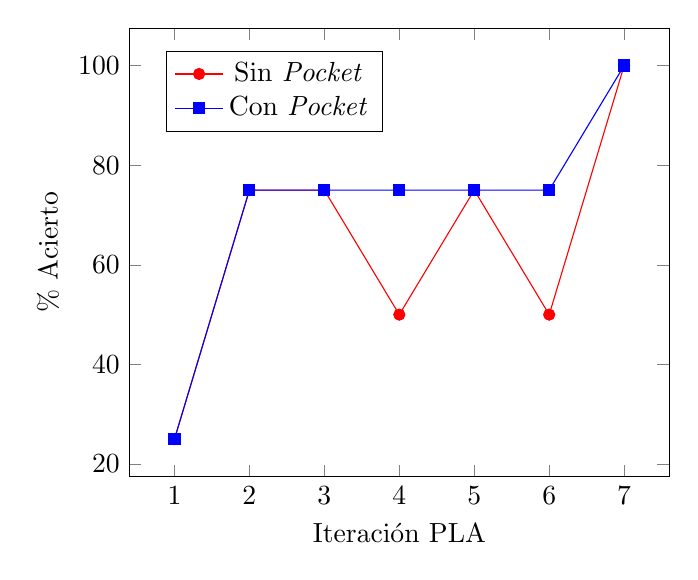
\begin{tikzpicture}
\begin{axis}[ xlabel=Iteración PLA, ylabel=\% Acierto, legend style={at={(0.47,0.95)}}]     \addplot[color=red,mark=*] coordinates
    {
    (1,25)
    (2,75)
    (3,75)
    (4,50)
    (5,75)
    (6,50)
    (7,100)
    };
    \addlegendentry{Sin \textit{Pocket}}
    
    \addplot[color=blue,mark=square*] coordinates
    {
    (1,25)
    (2,75)
    (3,75)
    (4,75)
    (5,75)
    (6,75)
    (7,100)
    };
    \addlegendentry{Con \textit{Pocket}}
\end{axis}
\end{tikzpicture}
\caption{Resultados del PLA con y sin \textit{Pocket}}
\label{plot:perceptronResultsWithAndWithoutPocket}
\end{figure}

Como ya hemos comentado, el algoritmo del \textit{Pocket} también podemos verle la utilidad en este sencillo experimento. En la figura \ref{plot:perceptronResultsWithAndWithoutPocket} se ve como a cada iteración que se ejecuta del PLA (también se puede ver como una época) dependiendo de si tenemos el algoritmo del \textit{Pocket} o no, al final obtendremos un resultado u otro. Esto es esencial cuando nos enfrentamos a un problema que no es linealmente separable y la mayoría de los problemas a los que se les puede aplicar el perceptrón y obtener unos resultados aceptables no serán linealmente separables.

\newpage
\subsection{Descripción de las tareas y trabajos desarrollados}


\newpage
\subsection{Descripción de los conocimientos y competencias adquiridos}


\newpage